\chapter{Teoretická část}
\label{chap:theoretical}
Reklamy se staly součástí životů většiny populace. Působí na lidskou mysl, přestože si to lidé nemusí ani uvědomovat.
Nasycené trhy dávají pro začínající podnikatele malou šanci úspěchu. Aby se mohli prosadit, musí nejen přinést světu jedinečný výrobek/službu,
ale musí umět svůj produkt také dobře reprezentovat a prosadit jej. Pro obchodníky se zavedenou tradicí a pozicí na trhu je zase nutné,
aby byly schopni své zákazníky udržet a nalákat nové. Pokud firma disponuje širokou nabídkou zboží,
vytváření grafické reklamy se stává časově náročnější.
Účelem této práce je prozkoumat možnosti automatizace jak tvorby, tak nasazení reklamy. 

V této kapitole jsou popsány základní pojmy týkající se marketingu a reklamy. Ve stručnosti jsou také popsány různé možnosti šíření reklamy
a srovnání jejich využitelnosti.

\section{Marketing}
\label{sec:marketing}
Účelem marketingu je poznávání, předvídání, ovlivňování a uspokojování potřeb a přání zákazníka způsobem, který je efektivní a výhodný a zajišťuje splnění
cílů organizace. Marketing vychází z trhu. Průzkum poptávky hraje důležitou roli v jeho efektivnosti.
Musí znát nejen momentální poptávku, ale také ji předvídat či přetvářet.

    \subsection{Marketingový mix}\label{ssec:marketing-mix}
    Marketingový mix je označení souhrnu základních nástrojů, které marketing využívá k dosažení cílů firmy.
    Existuje více alternativ marketingového mixu vycházejících z rozdílných pohledů na problém.
    Pohled ze strany podniku je označován jako 4P (z angl. Product, Price, Place, Promotion),
    zatímco z pohledu zákazníka se jedná o 4C (z angl. Customer value, Cost, Communication, Convenience).
    Tato práce se dále zabývá podnikovým mixem, konkrétně problému propagace.

    \subsection{Marketingová propagace}\label{ssec:marketing-propagation}
    \begin{quote}
        \enquote{\emph{Společenská praxe definuje pojem propagace jako uvedení něčeho nebo někoho v obecnou známost.
        Propagace v marketingovém pojetí je uvědomělá činnost, která informuje, přesvědčuje a ovlivňuje nákupní chování zákazníka.}}
        (SVĚTLÍK, J., 2016) \cite{svetlik:marketing}
    \end{quote}

    Marketingová propagace je součástí komunikačního mixu, který zahrnuje:
        \begin{itemize}
            \item podporu prodeje,
            \item reklamu,
            \item vztahy s veřejností,
            \item osobní prodej,
            \item přímý marketing.
        \end{itemize}
    Optimální strategii pro budování cíle komunikace zachycuje tzv. AIDA model. Ten zahrnuje tyto 4 kroky:
        \begin{enumerate}
            \item Získání pozornosti zákazníka.
            \item Vzbuzení zájmu.
            \item Vyvolat touhu po službě nebo produktu.
            \item Akce zákazníka.
        \end{enumerate}
    S propagací se úzce pojí \emph{cesta zákazníka}, která modeluje chování možných zákazníků na základě jejich vlastností,
    věku, osobností, trendů atd. Tento nástroj dokáže být velice užitečný v budování komunikační strategie tzn. reklamní slogany,
    cílovou skupinu, média pro šíření reklamy apod. 

    Pro efektivní propagaci je důležité, aby byla odrazem firemní identity. Firemní identita určuje způsob, jakým se firma prezentuje
    a to nejen vnějšímu světu ale také ve vlastních prostorách a ke svým zaměstnancům. Vizuální prvky firemní identity se obvykle doporučuje shrnout do
    jednoho dokumentu zvaný \emph{grafický manuál}.

    \subsection{Grafický manuál}\label{ssec:marketing-graphic-manual}
    Tento dokument přesně definuje vizuální elementy, kterými se organizace identifikují na otevřeném trhu.
    Součástí může být logo firmy, jeho různé barevné variace včetně návodů, jak je správně používat. V grafickém manuálu se specifikují textové fonty.
    Osvědčeným postupem je vybrat více fontů z důvodu dostupností na různých platformách. 

    Je doporučeno vybírat barvy podle standardizovaného vzorníku \emph{Pantone}. Důvodem je,
    že tyto barvy se na tištěném papíře velice podobat digitálním kopiím. Tiskárny a jejich subtraktivní barevný model CMYK totiž nedokáže přesně replikovat
    všechny barvy, které lze zobrazit počítačem. 

    Grafický manuál však může také obsahovat vzhled patičky internetové pošty, klasických papírových obálek,
    hlavičku a patičku dokumentů, ostatních tiskovin apod. 

    \section{Reklama}
    \begin{quote}
        \enquote{\emph{Ačkoliv reklama je pouze jedna z částí komunikačního (propagačního) mixu, je to část, která je nejvíce vidět.
        Mezi hlavní cíle reklamy patří kromě zvýšení poptávky a vyvolání nové či opakované koupě především tvorba silné značky,
        která zaujímá pevné a přední místo v mysli zákazníka mající k ní pozitivní postoj, dále identifikace a
        odlišení produktu (značky) od podobných produktů nabízených na trhu,
        vytváření pozitivní image firmy nebo výrobku a budování tak preferencí a věrnosti, posílení finanční pozice podniku,
        zvýšení možnosti distribuce a snížení nákladů spojených s prodejem, ale i motivace vlastních pracovníků aj.}}
        (SVĚTLÍK, J., 2016) \cite{svetlik:marketing}
    \end{quote}
    

    Síla reklamy se skrývá i ve schopnosti ovlivňování názorů lidí. Tohoto si lze nejčastěji všimnout např.
    u politických stran. Nejčastější reklamy lze podle způsobu použití dělit na 2 kategorie. \cite{marketing:product-vs-brand}

    \subsection{Produktová reklama}
    Tento druh reklamy je zaměřený na nabízený produkt, který se snaží vyzdvihnout výhody nad konkurencí.
    Jde o konkrétní nabízené služby nebo výrobky. Vhodné využití této reklamy je následující:
    \begin{itemize}
        \item Pokud je potřeba produktem oslovit velké publikum.
        \item Pokud je produkt skutečně \enquote{něčím dosud neviděným}.
        \item Pokud produkt \enquote{dokáže mluvit za sebe}.
    \end{itemize}

    \subsection{Značková reklama}
    Oproti produktové reklamě, se zde jedná spíše o zaujetí zákazníka jako takového. Nenabízí žádný konkrétní produkt,
    snaží se dostat zákazníkovi do podvědomí. Je výhodná pokud:
    \begin{itemize}
        \item Si značka chce vybudovat unikátní postavení na trhu. 
        \item Značka má zajímavý příběh o vzniku nebo historické pozadí. 
        \item Je prioritou budovat si zákaznickou důvěru značce. 
    \end{itemize}

    \subsection{Reklamní média}
    Jak tato práce výše zmiňuje, volba reklamního média závisí na cílové skupině, kterou se snaží oslovit.
    Správná volba dokáže pozitivně ovlivnit účinnost reklamy, zatímco špatný výběr může přinést pouze finanční zátěž.
    Média nejčastěji doručují význam reklamního sdělení 3 způsoby:
    \begin{enumerate}
        \item verbálně,
        \item zvukově,
        \item obrazově.
    \end{enumerate}
    Tato část práce rozebírá nejpoužívanější reklamní nosiče a jejich výhody. \cite{typy:medii} \cite{typy:mediatypy}
    
    \subsubsection{Tisk}
    Do této skupiny patří zejména periodické publikace jako noviny a časopisy. Tiskoviny jako katalogy, ročenky a zpravodaje zde lze také zařadit.
    Výhody tisku spočívají v geografickém zaměření -- možnost celostátního zaměření nebo jen jednotlivých regionů. Komerční sdělení se dá umístit k tématicky
    vhodným sekcím nebo časopisům. Zákazník při čtení novin a časopisů stráví více času na rozdíl od televize nebo rozhlasu,
    a proto mohou být sdělení obsáhlejší a komplexnější. Poslední výhodou jsou \emph{packshoty}, neboli společné balení inzerovaného produktu s magazínem.
    
    \subsubsection{Rozhlas}
    Rádia stejně jako noviny je možno použít pro možnost zaměření, a to nejen zeměpisným ale také časovým. Často se však stává,
    že se z rádia stane pouze kulisa na pozadí a člověk jej nevnímá. Působí pouze na jeden lidský smysl -– sluch,
    což pro nabízení určitých služeb či produktů nemusí stačit.

    \subsubsection{Outdoor}
    K této skupině se řadí jako nejpoužívanější média billboardy, citylighty, bigboardy, LED plochy a ostatní venkovní velké plochy nebo nápisy včetně
    firemních štítů, plakátů, MHD atd. Tyto nosiče setrvávají na svých místech a působí na lidi dlouhodobě, občas i vícekrát za den.
    Dají se zaměřovat od celostátního působení až na malá místa jako části měst. Nevýhodou je, že velice závisí na své lokalitě, viditelnosti a
    nemohou obsahovat složitá sdělení. 

    \subsubsection{Televize}
    Audiovizuální prezentace přes televize je jeden z nejúčinnějších prostředků komunikací s možným koncovým zákazníkem.
    Má široký rozsah uživatelů, dokáže nejlépe vyvolat emoce a asociace se značkou. Reklama se dá lépe cílit na základě měření sledovanosti.
    Její cena je však vysoká a je zde možnost, že si uživatel televize přepne kanál, aby nemusel reklamu sledovat.
    Navíc televizní inzerce se musí plánovat s předstihem z důvodů nepružných vysílacích plánů.
    
    \subsubsection{Kino}
    Ačkoli se tento typ média zdá nenápadným, má vysokou sledovanost. Divák je pohodlně usazen a v očekávání filmu věnuje svou pozornost všemu na promítacím plátně před sebou.
    Navíc je vše v perfektní kvalitě, jak zvukové, tak vizuální. Důležitým aspektem je vybrat kina s vysokou návštěvností a naplánovat reklamní kampaň předem, ideálně vložit spoty před promítání úspěšných projekcí.

    \subsubsection{Online}
    Internet je nejflexibilnější reklamní médium. Využívá jej velká část populace a rychle se rozrůstá. Nabízí různé možnosti inzercí, formátů,
    vysokou přesnost zaměření a jednoduchý monitoring. Jako jediný z výše zmíněných umožňuje interaktivní reklamu. Nabízí dobrou kontrolu nákladů a konverzí.
    Tři nejčastější způsoby platby jsou:
    \begin{itemize}
        \item PPV -- platba za zobrazení.
        \item PPA -- platba za nějakou akci (přihlášení k newsletteru, prodej, \ldots).
        \item PPC -- platba za proklik.
    \end{itemize}
    Internet přitáhl spoustu inzerentů a každý chce být co nejvíce viděn. Tímto vznikla vysoká konkurence mezi inzerenty, kdo zaplatí nejvíce za zobrazení své reklamy.
    Velký počet reklam na webu zase zapříčinil, že běžní uživatelé se chtějí reklamě vyhnout a snaží se jí blokovat.
    
    \subsubsection{Srovnání reklamních médií}
    Průzkum inzertních výkonů SPIR 2020 odhaluje, že i přes velké možnosti Internetu, je v České republice stále nejvíce investováno do reklamy televizní.
    Celkové srovnání medií se nachází na obrázku \ref{fig:spir-mediatypes}.


    \begin{figure}[h]
        \centering
        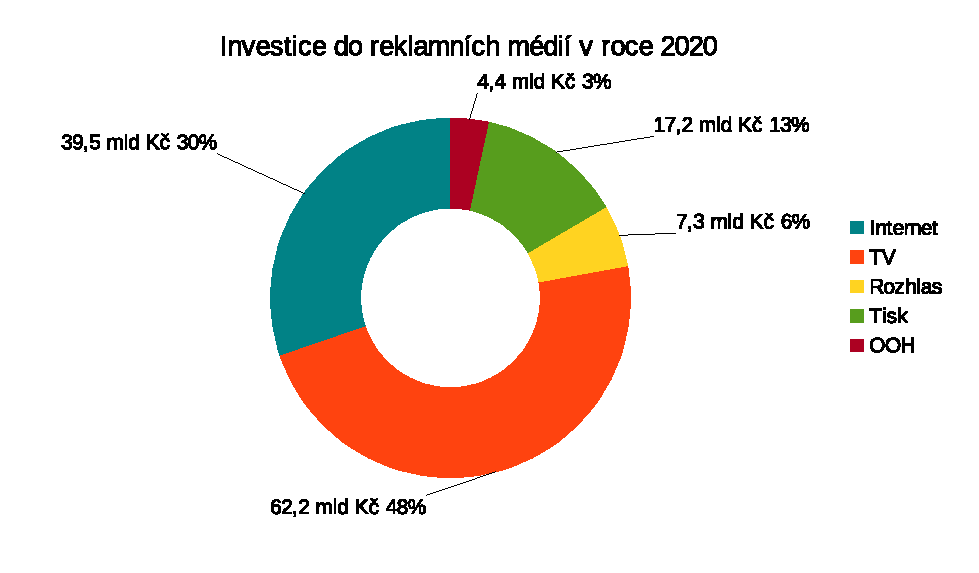
\includegraphics[width=0.9\textwidth]{Figures/pie-chart.eps}
        \iffalse
        This is my multi-line comment
        % \includesvg{Figures/pie-chart}
        % \begin{tikzpicture}
        %     \pie[
        %         text=pin,
        %         after number=~mld.,
        %         sum=auto,
        %     ]{39.5/Internet,
        %     62.2/TV,
        %     4.4/OOH,
        %     17.2/Tisk,
        %     7.3/Rozhlas}
        % \end{tikzpicture}
        \fi

        \caption[Podíl mediatypů v roce 2020]{Podíl jednotlivých mediatypů v roce 2020 \cite{spir:mediatypes}}
        \label{fig:spir-mediatypes}
    \end{figure}

    Možnosti online reklamy jsou velice rozsáhlé a stále se vyvíjejí. Následující kapitola se více zaměřuje na možnosti Internetové inzerce.

    \section{Internetová reklama}\label{sec:online-ad}
Moderní digitální doba nabízí mnoho způsobů, kterými lze komerční sdělení šířit. Jako jedny z hlavních forem se stává grafická (display) reklama,
reklama ve vyhledávání a emailová reklama. Nejčastějšími poskytovateli se stali sociální sítě a vyhledávače.
Obrovské množství denních uživatelů z nich udělali perfektní platformy pro nabízení inzercí.
Obrázek \ref{fig:spir-publishers} a tabulka \ref{tab:spir-publishers} zobrazují srovnání návštěvnosti 5 největších poskytovatelů online reklamy v České republice.

\begin{figure}[h]
    \centering
    \caption[Graf návštěvosti provozovatelů reklamních sítí]{Graf návstěvnosti reálných uživatelů provozovatelů reklamních sítí v ČR \cite{gemius:rating}}
    \label{fig:spir-publishers}
    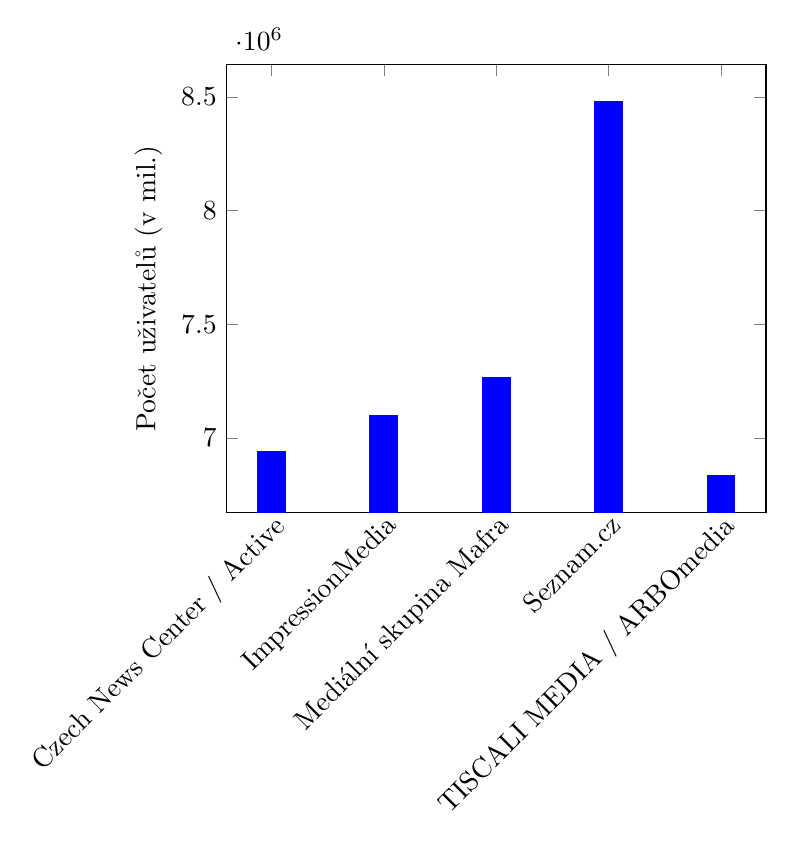
\begin{tikzpicture}
        \begin{axis}[
            symbolic x coords={Czech News Center / Active, ImpressionMedia, Mediální skupina Mafra, Seznam.cz, TISCALI MEDIA / ARBOmedia },
            x tick label style={rotate=45, anchor=north east, inner sep=0mm},
            xtick=data,
            ylabel=Počet uživatelů (v mil.),
          ]
            \addplot[ybar, fill, blue] coordinates {
                (Czech News Center / Active, 6938568)
                (ImpressionMedia,            7100320)
                (Mediální skupina Mafra,     7266377)
                (Seznam.cz,                  8480248)
                (TISCALI MEDIA / ARBOmedia,  6836590)
            };
        \end{axis}
    \end{tikzpicture}
    
\end{figure}

\begin{table}[hb]
    \centering
    \caption[Srovnání provozovatelů reklamních sítí]{Srovnání provozovatelů reklamních sítí \cite{gemius:rating}}
	\label{tab:spir-publishers}
    \begin{tabular}{l|r|r|r|r}
        \toprule
            Název & Reální uživatelé & Zobrazení stránky & Návštěvy & Čas \\
        \midrule
            Seznam.cz & 8 480 248 & 4 541 397 144  & 1 104 367 612 & 13782r 58d  \\
            Mediální skupina Mafra & 7 266 377 & 741 803 207  & 128 011 647  & 1156r 302d \\
            ImpressionMedia & 7 100 320  & 258 039 333 & 91 386 082 & 370r 7d  \\
            Czech News Center / Active & 6 938 568 & 508 776 721 & 110 070 333  & 549r 310d  \\
            TISCALI MEDIA / ARBOmedia & 6 836 590 & 120 326 836  & 44 648 445 & 204r 83d  \\
        \midrule
        
    \end{tabular}
\end{table}


Co se týče emailové reklamy, považuje se efektivní formu přímého marketingu, která je navíc zdarma.
Firmy mohou komunikovat se svými zákazníky jakožto stálými odběrateli nebo rozesílat hromadné emaily. Legislativně je však nevyžádaná elektronická pošta ošetřena.
Organizace tedy při posílaní emailů si musí být jisté, že je jejich sdělení oprávněné a nebude označeno jako spam.

Reklama ve vyhledávání se stává již placenou, většinou stylem PPC. Zadavatelé se za příplatek dostanou na první pozice výsledku hledání.
Toto jim zajišťuje vyšší míru prokliků a lépe nalákají potenciální zákazníky na svou webovou stránku. 

Grafická reklama (nejčastěji bannery a videa) je silným nástrojem pro rozšíření působnosti značky. Buduje povědomí o značce a
zároveň může lákat na produkt. Obsahuje reklamní sdělení, logo firmy a výzvu k akci (CTA) -- nejčastěji ve formě tlačítka.
Obrázek \ref{fig:spir-ad-performance} Ukazuje srovnání investic do grafické a vyhledávané reklamy.

\begin{figure}[h]
    \centering
    \caption[Výkon reklam v roce 2020]{Výkon jednotlivých forem internetové reklamy v roce 2020 \cite{spir:mediatypes}}
    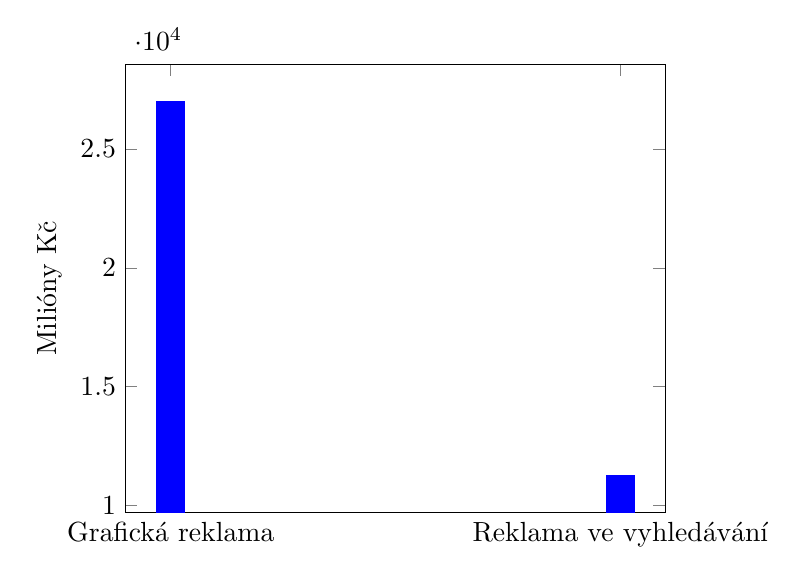
\begin{tikzpicture}
        \begin{axis}[
            symbolic x coords={Grafická reklama, Reklama ve vyhledávání},
            xtick=data,
            ylabel=Milióny Kč
          ]
            \addplot[ybar, fill, blue] coordinates {
                (Grafická reklama,           26998)
                (Reklama ve vyhledávání,     11274)
            };
        \end{axis}
    \end{tikzpicture}
    \label{fig:spir-ad-performance}
\end{figure}

    \subsection{Metriky internetových reklam}\label{ssec:online-ad-metrics}
    Jak tato práce již zmiňovala, výhodou online inzercí je jednoduchý monitoring. Na rozdíl od ostatních médií si firmy mohou být více jisté,
    že jejich reklamu cílené osoby opravdu vnímají. Hlavní metrikou reklamy vždy bývá zvýšení prodeje.
    Nicméně tato metrika se již měří obtížně a je spíše výsledkem z níže uvedených následujících ukazatelů.

        \subsubsection{Míra prokliku (CTR)}
        Takzvaná míra prokliku určuje, jak je velká šance že na reklamu někdo zareaguje kliknutím myši. Určuje se poměrem mezi celkovým počtem zobrazení reklamy a
        kliknutím na ni. Její význam spočívá v tom, že dokáže prozradit úspěšnost kampaně z hlediska upoutání pozornosti.

        \subsubsection{Míra okamžitého opuštění (BCR)}
        Tato metrika zaznamenává procento uživatelů, kteří se vlivem reklamy dostali na cílovou webovou stránku, ale neprovedou žádnou další aktivitu a
        typicky z webu odejdou. Vysoká procento BCR nejčastěji indikuje jednu z následujících věcí:
        \begin{itemize}
            \item Cílová webová stránka byla nízké kvality. Např. nezajímavý vzhled, neresponzivnost, nepřístupnost, dlouhá doba načítání atd.
            \item Produkt nebo služba nabízená v reklamě nesouvisí s tím, co člověk hledal.
            \item Osoba na stránce našla vše potřebné a další informace nepotřebuje.
        \end{itemize}

        \subsubsection{Konverzní poměr (CVR)}
        Konverzní poměr je výsledkem osob, kteří skrze reklamu dostali na webovou stránku, dokončili nějakou akci (a stali se tak zákazníky) s
        celkovým počtem zobrazení stránky. Akci, kterou mají uživatelé splnit si firma určí sama. Pro e-shopy toto může znamenat dokončení objednávky,
        pro blogy třeba přehlášení k newsletteru.

        \subsubsection{Návratnost investic (ROI)}
        Inzerování je spjato s náklady a investicí. Ve své nejjednodušší podstatě je poměr nákladů a výdělku výslednou metrikou.
        Výdělkem nemusí být pouze zisk, ale i jiný cíl, který si firma stanoví (zvýšení popularity, uživatelů atd.).

    \subsection{Zobrazení online reklamy}
    Pro dobré využití reklamy je potřebné jej umístit na dobře viditelná místa webových stránek s vysokou návštěvností.
    Těmi se stali převážně sociální sítě typu Facebook, Youtube, Twitter apod. Jelikož tito giganti vlastní i více dalších podobných stránek,
    vznikly reklamní sítě jako Google Ads. To umožnilo vznik partnerských webů, které zobrazují reklamy právě prostřednictvím těchto sítí.
    Na oplátky dostávají partnerské weby část tržby ze zobrazených reklam.

    Zmiňované reklamní sítě mají za úkol dát správnou reklamu na správný web.
    Korektní stránku lze vybrat na základě jejího celkového obsahu, klíčových slov vyhledávání spotřebitele či dokonce z analýzy způsobu prohlížení stránky.
    Inzerenti si kupují \enquote{online prostor} pro svou reklamu. 

    Druhou možností je \enquote{kupovat} si cílové publikum své reklamy, a to za pomocí technologie \emph{RTB}.
    Na začátku si inzerent při tvorbě reklamní kampaně vybere svou cílovou skupinu. Tu specifikuje pomocí různých demografických kritérií apod.
    Ve zjednodušené podobě je průběh RTB znázorněn na obrázku \ref{fig:rtb}.

    \begin{figure}[h]
        \centering
        \caption[Fungování RTB]{Zjednodušený způsob fungování RTB \cite{rtb}}
        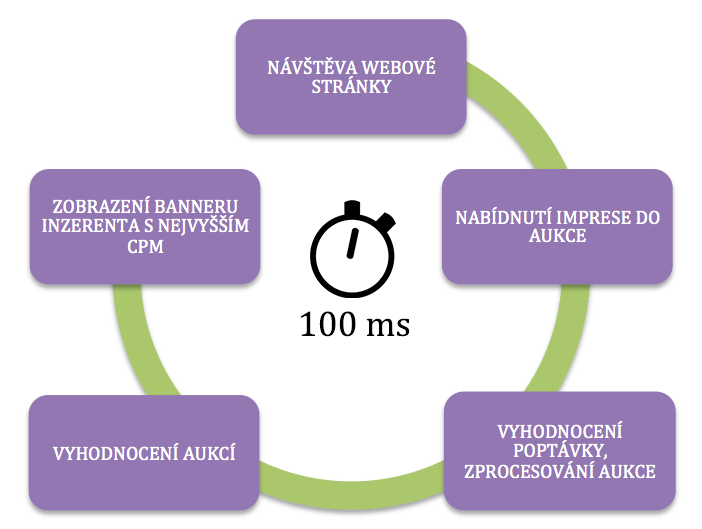
\includegraphics[width=0.7\textwidth]{Figures/rtb.png}
        \label{fig:rtb}
    \end{figure}

\endinput

    \section{Bannerová reklama}
    \begin{quote}
        \enquote{\emph{Cílem bannerové reklamy je nejen zprostředkovat reklamní sdělení, ale i zabezpečit, aby se recipient velmi jednoduchou aktivitou
        (kliknutím na banner) přesunul na požadovanou webovou lokalitu (firemní stránku, stránku značky, stránky produktu/značky na sociální síti atd.).}}
        (SVĚTLÍK, J., 2017) \cite{svetlik:reklama}
    \end{quote}

    V této části se práce více zaměřuje na bannerovou reklamu.
    Teorie a efektivita tohoto typu inzerce je zde rozebrána jako první a více do detailu. \cite{banner:advertising}

    \subsection{Formáty zobrazení}
    První webový banner se objevil na internetu v roce 1994. V té době se bannery objevovali nejčastěji jako statický obrázek ve formátu
    JPEG nebo PNG. Tento způsob zobrazení se udržel dodnes. Dynamický obsah v podobě animace bylo schopný zobrazit formát GIF a to v podobně pohyblivých obrázků.
    Společnost Macromedia s jejich technologií \emph{Flash} dokázali do bannerů přidat i možnosti interakce v podobě animací nebo přehrání zvuku při
    pohybu kurzoru myši nad bannerem. Dnes už technologie Flash z důvodu bezpečnosti a HW nároků není ve významných internetových prohlížečích podporována a
    dá se plně nahradit spojením HTML a JS kódu. 

    \subsection{Statický nebo dynamický banner}
    Statický banner je pouhým obrázkem, který se nijak nehýbe a nemá možnost interakce s uživatelem. S nástupem bannerů na Internet se u
    spotřebitelů začal objevovat fenomén zvaný \emph{bannerová slepota}. Bylo zjištěno, že někteří uživatelé podvědomě bannery na standardních místech
    úplně ignorují a nevnímají je. Proti tomuto jevu dokáži efektivně bojovat dynamické bannery.
    I krátká animace dokáže zachytit pozornost oka a tím lépe působit na cílové publikum.
    Toto se dá jednoduše změřit při porovnání CTR statických a dynamických bannerů.

    \subsection{Rozměry bannerů}
    Některé ze standardních rozměrů bannerů (v px) a jejich názvy lze vidět na obrázku \ref{fig:banner-sizes}. Podle rozlohy se zobrazují na jiných částech webových stránek nebo
    mobilních aplikací. S rozměry se také pojí velikost souborů. Reklamní sítě mívají na nahrané bannery limity velikostí.
    Čím menší velikost, tím rychleji se dokáže banner načíst. Nejčastější limit bývá 150~KB. Toto je více rozebráno v kapitole o reklamních sítích.

    \begin{figure}[h]
        \centering
        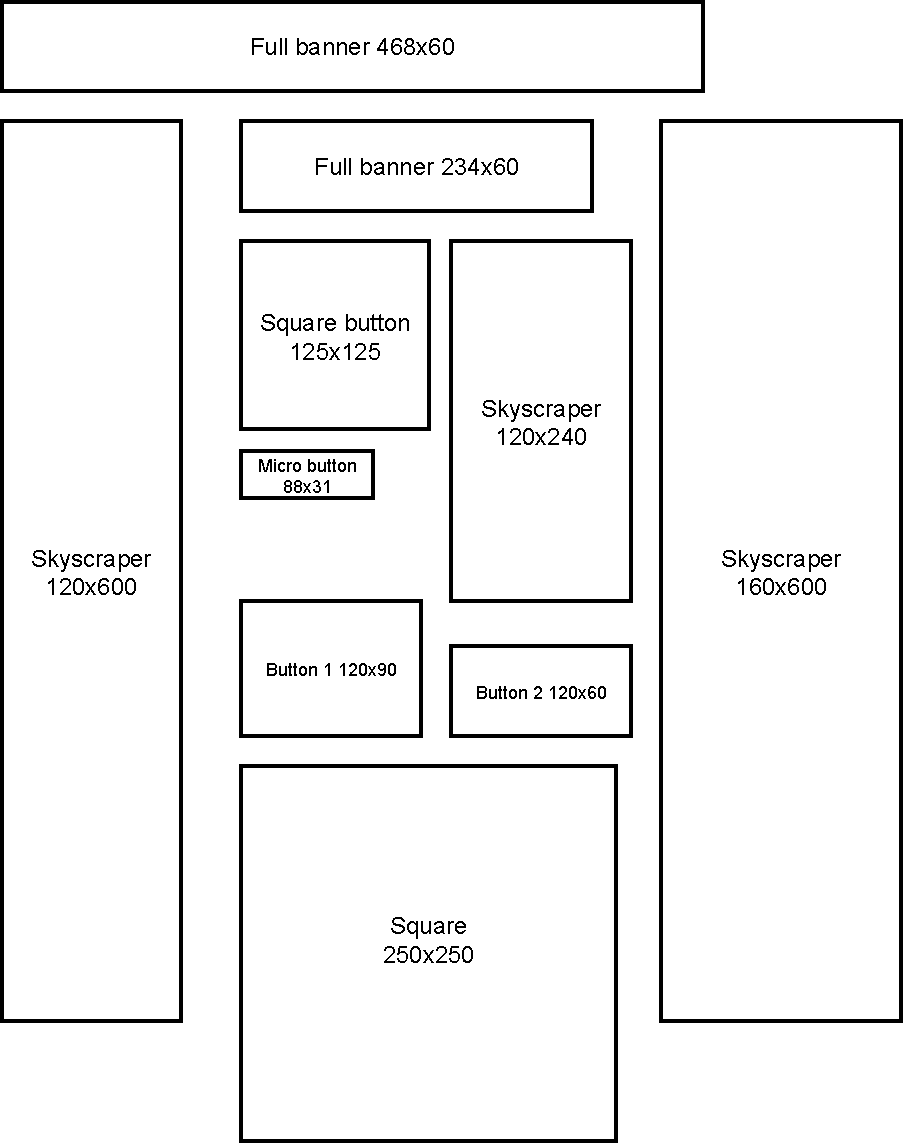
\includegraphics[width=1\textwidth]{Figures/banner-sizes.pdf}
        \caption[Velikosti bannerů]{Standardní používané velikosti bannerů}
        \label{fig:banner-sizes}
    \end{figure}

    \subsection{Jak vytvořit dobrý banner}
    Jak měřit efektivitu reklamy se zmiňuje část \ref{ssec:online-ad-metrics}. Tato část se věnuje tomu, jak banner vytvořit,
    aby již zpočátku co nejvíce upoutal zákazníky. \cite{banner:design}
    Reklamní banner se skládá ze 4 základních částí. Těmi jsou:
    \begin{itemize}
    \item logo inzerenta,
    \item titulek (komerční sdělení),
    \item pozadí,
    \item výzva k akci (CTA).
    \end{itemize}
    Na banneru se může nacházet více prvků, je však důležité, aby tyto hlavní části splnily doporučená pravidla, která jsou zde postupně rozebrána.

    \subsubsection{Logo}
    Pokud je to možné, mít logo na banneru je velice důležité. Pomáhá budovat povědomí o značce a napovídá zákazníkovi na čí webovou stránku by se měl dostat.
    Mělo by být dobře viditelné, ale nemělo by opticky přebíjet titulek nebo výzvu k akci.

    \subsubsection{Pozadí}
    Co se pozadí týče, na výběr jsou 2 varianty. Buď celobarevné nebo fotografie. Obojí má svá pro i proti. Pokud se banner snaží prodat nějaký produkt,
    je vhodnější vynechat obrázkové pozadí. Jednobarevná pozadí vytváří přirozený kontrast s výzvou k akci.
    Produkt na ni dobře vynikne a neodvádí pozornost od titulku. Naproti tomu, pokud se vytváří reklama na určitou službu nebo
    produkt nefyzického charakteru (nejčastěji software, IT služby) lze fotografií na pozadí ilustrovat onu nabízenou věc. 

    \subsubsection{Titulek}
    Doporučuje se spíše krátký text. Za úkol má přilákat pozornost možného zákazníka, tím pádem rozměrově zabírá větší část banneru.
    Podstatné kritérium je, aby byl text opět dobře čitelný. Proto je zapotřebí zvolit kontrastní barvu textu s dobře čitelným fontem.
    Řez písma by neměl být příliš tenký, jinak by text mohl splývat s pozadím nebo se špatně číst. Efekty typu zkosení se moc nedoporučují a
    někteří poskytovatelé reklamních sítí je vůbec nepovolují. 

    \subsubsection{Výzva k akci}
    Měla by u diváka vyvolat pocit nutnosti na banner kliknout. Zároveň by měla být dobře viditelná hned po titulku.
    Proto se často vyskytuje v podobě tlačítka s vhodně zvolenou barevnou kombinací.
    Umístění blíže k titulku diváka přirozeně navede.


\endinput

    \section{Poskytovatelé reklamních sítí}
\label{sec:networks}
Jak tato práce již zmiňovala, reklamám se nejlépe daří na webových stránkách s vysokou návštěvností, protože se inzerce zobrazí více návštěvníkům.
Tato část si podrobněji rozebere a porovná podmínky online bannerové reklamy od několika různých poskytovatelů. 

    \subsection{Google}
    Tento web se stal králem Internetových vyhledávačů. S průměrem kolem 3,5 miliónů vyhledávacích dotazů za minutu (celosvětově),
    jen potvrzuje své dominantní postavení. Reklamu poskytuje v rámci své služby Google Ads (dříve Google AdWords),
    která nabízí vyhledávací kampaně, obsahové kampaně a video kampaně. Co se týče bannerové reklamy,
    Google podporuje 3 formáty obrázkových souborů (PNG, JPEG, GIF) standardních specifikovaných velikostí, které řadí do 4 kategorií:
    \begin{itemize}
        \item čtvercové a obdélníkové,
        \item svislé,
        \item výsledková tabule,
        \item mobilní.
    \end{itemize}

    Lze nahrát archiv ZIP obrázků, který nesmí mít více než 40 souborů celkem a všechny obrázky musí být do max 150 KB. V případě že se jedná o GIF animaci,
    nesmí přesáhnout 30 vteřin. Zároveň v animacích nesmí být blikající efekty a frekvence snímků nesmí překročit 5 snímků za vteřinu.

    Za zmínku také stojí možnost tzv. Responzivní reklamy. Ta funguje tak, že inzerent si nahraje svá loga, produkty,
    doplní titulek a ostatní informace. Potom Google za použití strojového učení sám dynamicky sestavuje a zobrazuje kompletní bannery.
    Ovšem při tomto použití nemá inzerent plnou kontrolu nad výslednou grafikou.

    Ohledně reklamní politiku Googlu, nedovoluje propagaci padělaného zboží, nebezpečných produktů a služeb včetně tabákových výrobků,
    nevhodného a nemorálního obsahu jako např. šikana, zastrašování, vydírání, hackování, falešné dokumenty a plagiátorství. Dále, pokud osoba,
    která chce své produkty inzerovat nesmí zneužívat reklam k obsahu, který slouží pouze k navedení na koncového zákazníka někam jinam,
    shromažďovat uživatelská data k neznámým nebo nekalým účelům nebo se vydávat za někoho jiného. S určitým omezením a ohledem na zákony či věk svých koncových
    uživatelů dovoluje Google reklamy na erotický obsah, alkohol, hazardní hry, politický obsah, finanční služby, zdravotnické služby a léky.

    \subsection{Facebook}
    Facebook společně s Instagramem podporují velké množství obrázkových formátů. Ale pro nejlepší výsledky doporučují JPEG nebo PNG.
    Tento poskytovatel nezobrazuje standardní bannery, ale pouze obrázky, u kterých záleží na poměru stran.
    Velikosti a poměr stran obrázků se odvíjí podle toho, kam chceme reklamu mít umístěnou. Podporované poměry stran jsou tyto:
    \begin{itemize}
        \item 1,91:1,
        \item 16:9,
        \item 1:1,
        \item 4:5,
        \item 2:3,
        \item 9:16.
    \end{itemize}

    Každý z poměrů stran je vhodný pro zobrazení na různých místech těchto sociálních sítí (např. Kanál příspěvků, Stories, atd.).
    Kompletní tabulku je možno najít na tomto \href{https://www.facebook.com/business/help/682655495435254?id=271710926837064}{odkazu.}

    Minimální doporučené rozlišení je 1080x1080px. Oproti Googlu může být soubor velký až 30 MB.
    Reklamy na Facebooku a Instagramu musí být v souladu se zásady komunity, musí odkazovat na plně funkční úvodní stránky,
    nesmí obsahovat nezákonné produkty nebo služby, diskriminační postupy, nebezpečné doplňky stravy, tabák a s ním související produkty,
    obsah pro dospělé, dezinformace atd.

    \subsection{Sklik}
    Česká služba Sklik firmy Seznam.cz si v České republice vybudovala podobné postavení jako Google.
    Dle dat firmy Gemius, je Seznam.cz největším vydavatelem online reklamy v České republice. Pro lepší inzerci poskytuje cílení
    např. podle témat partnerských webů, zájmů uživatelů, pohlaví, klíčových slov atd.

    Povolené soubory pro nahrání bannerové reklamy jsou PNG, JPEG a GIF. Velikostně se soubory musí vlézt do max. 150 KB a
    rovněž podporuje všechny standardní velikosti bannerů.

    Bannery musí vyplňovat celou reklamní plochu, musí být jasně čitelné, relevantní, obsahově a kvalitativně srozumitelné.
    Také by měli mít textové sdělení -- krátký popis nebo výzva k akci. Reklama nesmí napodobovat, nesmí porušovat autorská práva,
    je zakázáno používat clickbaitové sdělení typu \enquote{Budete v šoku} apod. Reklama na erotický obsah se zobrazuje pouze od 22:00 do 6:00.  

\endinput




\endinput